\chapter*{Part One: Matrix Factorization}
\addcontentsline{toc}{chapter}{Part One}

The first part to code was the latent semantic analysis word representations. Latent semantic analysis uses singular value decomposition to represent words in a lower dimensional space than the number of documents in the corpus. In my case, I found that using the principle components matrix $\bm{U}$ alone provided significantly better results than weighting it with the diagonal matrix $\bm{\Sigma}$.

\begin{python}
    def learn_reps_lsa(matrix, rep_size):
    U, sigma, V = np.linalg.svd(matrix, full_matrices=True)
    return result = U[:, :rep_size]
\end{python}

The next piece of code is the term frequency-inverse document frequency (TF-IDF), which re-weights word counts in the term-document matrix to prevent frequent words from dominating the word representation. It penalizes ubiquitous words while allowing sparser data to appear in the representation.

\begin{python}
    def transform_tfidf(matrix):

    nwords, ndocs = matrix.shape
    vidf = np.vectorize(idf_helper)
    idfs = np.zeros(nwords)
    for i, _ in enumerate(idfs):
    idfs[i] = idf_helper(matrix[i,:], ndocs)
    tfidf = np.multiply(matrix, idfs[:, np.newaxis])
    return tfidf

    def idf_helper(row, ndocs):
    df = np.count_nonzero(row)
    idf = np.log(ndocs/df)
    return idf
\end{python}

The final code is the LSA featurizer, which projects word contexts into the LSA lower dimensional representation.

\begin{python}
    def lsa_featurizer(xs):
    lsa = reps_tfidf
    feats = xs @ lsa
    # normalize
    return feats / np.sqrt((feats ** 2).sum(axis=1, keepdims=True))
\end{python}

\subsection*{Theoretical Problem A}
The singular value decomposition of a matrix $\bm{M}$ is given by

\begin{equation*}
    \bm{M} = \bm{U \Sigma V}
\end{equation*}

Given the word co-occurence matrix $\bm{W_{tt}} = \bm{W_{td}W_{td}^T}$ we can solve as follows by applying the SVD to the matrix and its transpose:

\begin{align*}
    \bm{MM^T} & = \bm{U \Sigma V^T} \cdot \bm{V \Sigma U^T} \\
              & = \bm{U \Sigma^2 U^T}
\end{align*}

The final result is itself a singular decomposition, where the left singular matrix of $\bm{W_{tt}}$ is equal to the left singular matrix of the original term-document matrix $\bm{W_{td}}$.
If $\bm{U}$ is negative, then $\bm{U \Sigma^2 U^T}$ is positive, resulting in flipped signs compared to the original, therefore the left singular matrices are equivalent to each other's absolute values. This behavior is observed in my implementation of learn\_reps\_lsa, which simply truncates $\bm{U}$ along its second axis to achieve a lower dimensional word representation. This implies that word co-occurence relations can be incorporated while using $\bm{U}$ for my representation.

\subsection*{Experimental Problem B}

The nearest neighbors in representation space appear better for some words than others. For instance, their is a clear connection between dog and all of its top related words. Words associated with "the" are seemingly random; given that "the" is a filler word, associations are likely largely meaningless.

For this data set, using a smaller representation size and therefore a denser approximation of the term-document matrix appears to give slightly more meaningful associations.

\begin{tabular}{ |p{3cm}|p{3cm}|p{3cm}|p{3cm}|  }
    \hline
    \multicolumn{4}{|c|}{Word Similarities r = 100}                 \\
    \hline
    the             & dog            & 3           & good           \\
    \hline
    lid 1.753       & foods 0.571    & per 0.884   & pretty 1.255   \\
    leaked 1.779    & pets 0.624     & 1 0.943     & bread 1.349    \\
    filter 1.779    & switched 0.742 & 2 0.992     & prepare 1.376  \\
    rest 1.786      & pet 0.794      & 4 1.061     & flaxseed 1.407 \\
    flavoring 1.789 & cheap 0.831    & ounce 1.100 & beat 1.457     \\
    \hline
\end{tabular}

\begin{tabular}{ |p{3cm}|p{3cm}|p{4cm}|p{3cm}|  }
    \hline
    \multicolumn{4}{|c|}{Word Similarities r = 500}                     \\
    \hline
    the           & dog            & 3                 & good           \\
    \hline
    suspect 1.953 & happier 1.670  & omega 1.733       & gerber 1.873   \\
    flowers 1.961 & earlier 1.681  & vendor 1.739      & luck 1.885     \\
    leaked 1.966  & eats 1.702     & supermarket 1.747 & crazy 1.890    \\
    m 1.966       & stays 1.722    & nutty 1.755       & flaxseed 1.907 \\
    burn 1.967    & standard 1.727 & carries 1.797     & suspect 1.907  \\
    \hline
\end{tabular}

\subsection*{Experimental Problem C}

\chapter*{Part Two: Language Modeling}
\addcontentsline{toc}{chapter}{Part Two}

This section of the assignment involved implementing a Word2Vec model. My model uses CrossEntropy as its loss function for training, as we are training the model to predict binary labels for positive or negative reviews. CrossEntropy increases loss as a prediction is a further distance from the actual label, making it suited for teaching a model to label a review as good or bad.

For my model itself, I used the standard PyTorch embedding module to represent words. In my forward function, I sum the embedding of all context words for the CBOW model, put the embeddings through a linear layer, and then a log softmax.

I've observed some variance in my training. Somewhere a random number isn't seeded, so the finaly accuracy varies between different trainings in the range of ~.8 to .825.

\subsection*{Experimental Problem A}

The nearest neighbor space for Word2Vec is entirely unintuitive to me. The associated words for good seem reasonable, but every other example word seems somewhat random (particularly dog and barbecue). However Word2Vec appears to be my strongest featurizer, so perhaps the model is learning relationships that are not evident to me? In a production system I would worry it is cheating somehow and discovering idiosyncrasies hidden in my training set.

\begin{tabular}{ |p{3cm}|p{3cm}|p{4cm}|p{3cm}|  }
    \hline
    \multicolumn{4}{|c|}{Word2Vec Word Similarities context  = 2}    \\
    \hline
    the         & dog             & 3                 & good         \\
    \hline
    lots 1.668  & companies 1.686 & sip 1.701         & nice 1.660   \\
    fish 1.752  & double 1.707    & gingerbread 1.734 & sauces 1.697 \\
    betty 1.771 & barbeque 1.713  & pets 1.7434       & pure 1.698   \\
    alive 1.774 & times 1.717     & send 1.750        & great 1.704  \\
    my 1.775    & leak 1.726      & bears 1.752       & photo 1.732  \\
    \hline
\end{tabular}
\subsection*{Experimental Problem B}
Word2Vec is consistently about 2\% more accurate than any of my other featurizers.

\subsection*{Experimental Problem 3}
In terms of accuracy for my downstream task, two appears to be the magic number for my Word2Vec implementation. Using a context size of one tanks the model performance, and increasing it beyond two more gradually decreases performance.

Using a larger context size increases the distance from the center word that our model examines when learning. The relationships between words become less intuitive as the model is more likely to pick up on words farther away in the sentence. For instance, with a context size of six, dog has the following related words: junk, intake, photo, replace, and generally. One could imagine a review along the lines of "Generally I feed my little dog smaller kibbles" that is causing the adverb generally to associate with dog.



% \begin{figure}[h]
%     \centering
%     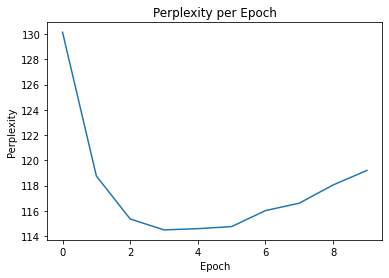
\includegraphics[width=0.4\textwidth]{resources/png/no_bias_1e3.png}
%     \noskipcaption{Perplexity of a vanilla RNN over 10 epochs with learning rate 1e-3}
%     \label{firsttry}
% \end{figure}



\chapter*{Part Three: Improving the Model}
\addcontentsline{toc}{chapter}{Part Three}

\chapter*{Part Four: Skip-Gram Variant}
\addcontentsline{toc}{chapter}{Part Four}




\subsection*{Theoretical Problem A}
\begin{equation*}
    \sigma(\vec{w} \cdot \vec{c})=\frac{1}{1+e^{-\vec{w} \cdot \vec{c}}}
\end{equation*}

Substituting $x$ for $\vec{w} \cdot \vec{c}$

\begin{equation*}
    \frac{\partial \log \sigma(x)}{\partial x} = 1 - \frac{1}{e^{-x}+1}
\end{equation*}

\subsection*{Theoretical Problem B}

Given the local objective function

\begin{equation*}
    \ell(w, c)=\#(w, c) \cdot \log \sigma(\vec{w} \cdot \vec{c})+k \cdot \#(w) \cdot \frac{\#(c)}{|D|} \cdot \log \sigma(-\vec{w} \cdot \vec{c})
\end{equation*}

Again substituting $x$ for $\vec{w} \cdot \vec{c}$, and substituting $\lambda$ for the constant expression $k \cdot \#(w) \cdot \frac{\#(c)}{|D|}$ and $\alpha$ for constant term $\#(w,c)$

\begin{align*}
    \frac{\partial \ell(x)}{\partial x} & = \frac{\alpha}{e^x + 1} -\lambda \frac{e^x}{e^x + 1}
\end{align*}

Setting the derivative to $0$ we can rewrite $\partial \ell$ in the form

\begin{align*}
     & \frac{\alpha}{1 + e^x} = \frac{\lambda e^x}{1 + e^x}             \\
     & \frac{\alpha}{\lambda} = e^x                                     \\
     & x = \log(\frac{\alpha}{\lambda})                                 \\
     & =\log \left(\frac{\#(w, c)}{\#(w) \cdot \#(c) k} \cdot|D|\right)
\end{align*}

\subsection*{Theoretical Problem C}
Pointwise mutual information is the ratio of how often two events (in our case a word and its context) occur together versus how often they could be expected to occur if one assumes the events are independent. It is a useful index for showing quantitatively how strongly words are associated with each other.

The critical points of the skip-gram local objective function are the same as the PMI formulation except scaled by a factor of $\log(1/k)$. $k$ is the number of negative samples introduced to each context. WHen $k=1$, the skip-gram model trains our embedding vectors towards exactly the PMI.

\chapter*{Appendix}
\subsection*{Vanilla RNN}
\begin{python}
    import os
\end{python}

